\documentclass[a4paper]{article}
\usepackage[procnames]{listings}
\usepackage{color}
\usepackage{graphicx}

\begin{document}
\definecolor{keywords}{RGB}{255,0,90}
\definecolor{comments}{RGB}{0,0,113}
\definecolor{red}{RGB}{160,0,0}
\definecolor{green}{RGB}{0,150,0}
\lstset{language=Python, 
        basicstyle=\ttfamily\small, 
        keywordstyle=\color{keywords},
        commentstyle=\color{comments},
        stringstyle=\color{red},
        showstringspaces=false,
        identifierstyle=\color{green},
        procnamekeys={def,class}}

\title{EM Algorithm}
\author{Bochen Wang, Tianyuan Liu}
\maketitle
\section*{Introduction}
This is the second part of Homework 3. Implement the EM algorithm. \\
Problem (a) is explained in the writing exercise 14.2.
\section*{Implementation}
\subsection*{Read Data}
Read data from faithful.dat and normalize the data into 0 to 1. Plot the data points.
\begin{lstlisting}

def read_data():
    data = []
    with open('faithful.dat') as filein:
        for line in filein:
            currline = line.strip('\n')
            data.append(currline)
    data = data[-272:]
    temp = []
    for e in data:
        record = e.split()[1:]
        record[0] = float(record[0])
        record[1] = float(record[1])
        temp.append(record)
    data = np.array(temp)
    min_max_scaler = preprocessing.MinMaxScaler()
    data[:,0] = min_max_scaler.fit_transform(data[:,0])
    data[:,1] = min_max_scaler.fit_transform(data[:,1])
    # print data    
    return data
    
def plot_fig(data):
    nullfmt = NullFormatter()
    x, y = data[:,0],data[:,1]
    left, width = 0.1, 0.65
    bottom, height = 0.1, 0.65
    bottom_h = left_h = left + width + 0.02
    
    rect_scatter = [left, bottom, width, height]
    rect_histx = [left, bottom_h, width, 0.2]
    rect_histy = [left_h, bottom, 0.2, height]
    
    plt.figure(1, figsize=(8, 8))

    axScatter = plt.axes(rect_scatter)
    plt.xlabel("eruptions")
    plt.ylabel("waiting")
    axHistx = plt.axes(rect_histx)
    axHisty = plt.axes(rect_histy)
    axHistx.xaxis.set_major_formatter(nullfmt)
    axHisty.yaxis.set_major_formatter(nullfmt)
    
    axScatter.scatter(x, y)
    
    # now determine nice limits by hand:
    axHistx.hist(x, bins=20)
    axHisty.hist(y, bins=20, orientation='horizontal')
    
    plt.savefig('Scatter_Plot.png')
    plt.show()
    
\end{lstlisting}
\begin{center}
	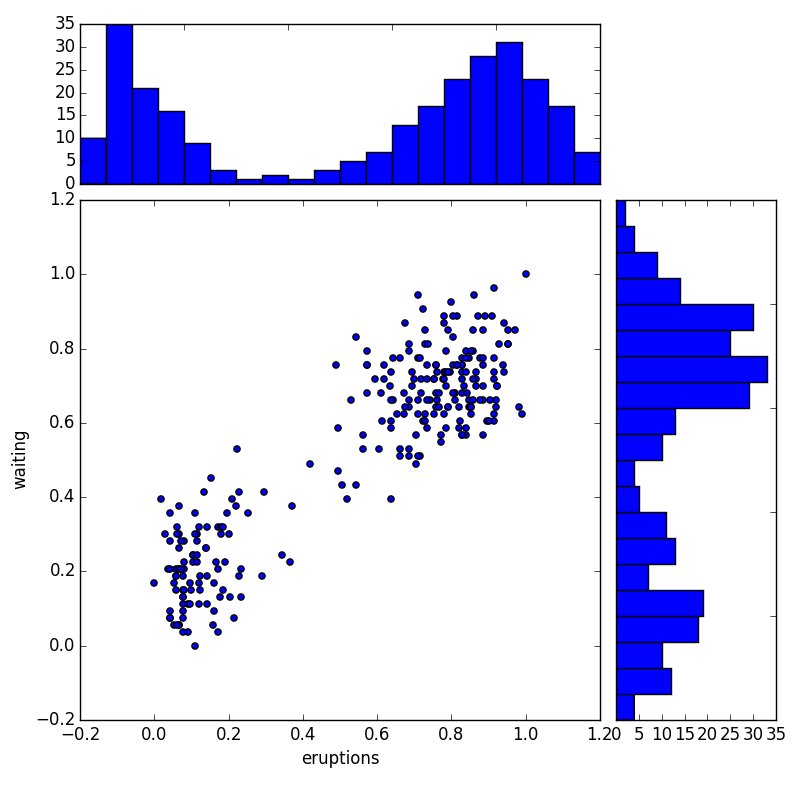
\includegraphics[scale=0.6]{Scatter_Plot}
\end{center}

\subsection*{EM algorithm}
Implement EM algorithm with randomly initialized Gaussian parameters.
\begin{lstlisting}
def random_init(x):
    random.seed(None)
    n,p = x.shape
    
    # random initialize pis
    pi = random.random()
    pis = [pi,1-pi]
    # print pis

    # random initialize mus
    mus = np.zeros((2,p))
    for i in xrange(p):
        for j in xrange(2):
            mus[j,i] = random.random()
    # print mus

    # random initialize sigmas
    sigmas = np.zeros((2,p,p))
    for j in xrange(2):
        for i in xrange(p):
            sigmas[j,i,i] = 0.5+random.random()*10
    # print sigmas
    return pis,mus,sigmas

# pis = [pi,1-pi] mus = [mu1, mu2] sigmas = [sigma1, sigma2]
# tolerance = 0.0001 default, max iteration = 100 default 
def EM_algo(x,pis,mus,sigmas,tol=0.0001,maxiter=100):
    # n denotes oberservation count, p denotes oberservation dimension
    n, p = x.shape
    # k denotes normal distrubutions count  
    k = len(pis)
    # ll_old denotes old log likelyhood
    ll_old = 0
    iter_count = 0
    mu_vector = []
    mu_vector.append(mus)
    for i in xrange(maxiter):
        iter_count += 1
        # E-step
        ts = np.zeros((k,n))
        for j in xrange(k):
            for i in xrange(n):
                ts[j,i] = pis[j] * mvn(mus[j],sigmas[j]).pdf(x[i])
        ts /= ts.sum(0)
        
        # M-step
        # update pi
        pis = np.zeros(k)
        for j in xrange(k):
            for i in xrange(n):
                pis[j] += ts[j,i]
        pis /= n

        # update mu
        mus = np.zeros((k, p))
        for j in xrange(k):
            for i in xrange(n):
                mus[j] += ts[j, i] * x[i]
            mus[j] /= ts[j, :].sum()
        mu_vector.append(mus)
        # update sigma
        sigmas = np.zeros((k,p,p))
        for j in xrange(k):
            for i in xrange(n):
                ys = np.reshape(x[i]- mus[j], (2,1))
                sigmas[j] += ts[j, i] * np.dot(ys, ys.T)
            sigmas[j] /= ts[j,:].sum()

        ll_new = 0.0
        for i in xrange(n):
            s = 0
            for j in xrange(k):
                s += pis[j] * mvn(mus[j], sigmas[j]).pdf(x[i])
            ll_new += np.log(s)

        if np.abs(ll_new - ll_old) < tol:
            break
        ll_old = ll_new
    mu_vector = np.array(mu_vector)
    # print iter_count, mus
    return iter_count,mu_vector,pis,mus,sigmas
    
\end{lstlisting}
Plot the mean vectors trajectories. \\
\begin{center}
	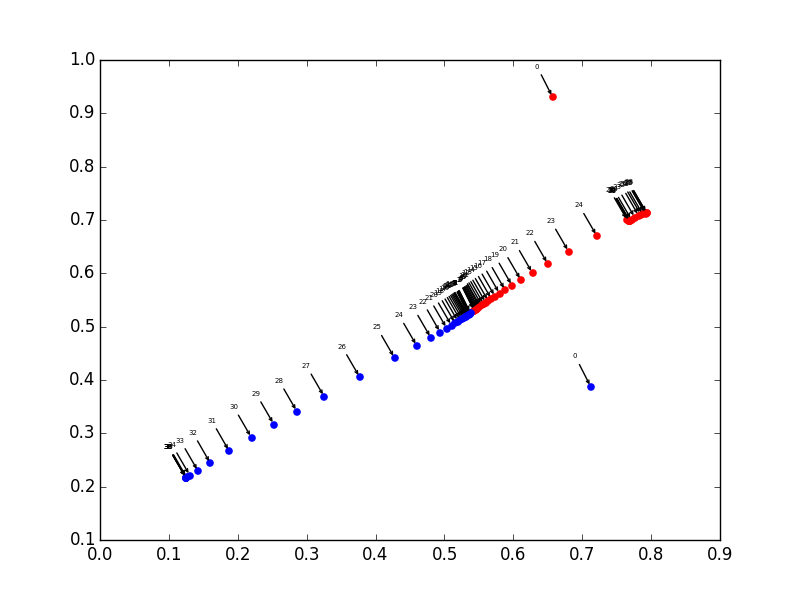
\includegraphics[scale = 0.6]{Mean_Trajectory}
\end{center}
Plot the iterations histogram. \\
\begin{center}
	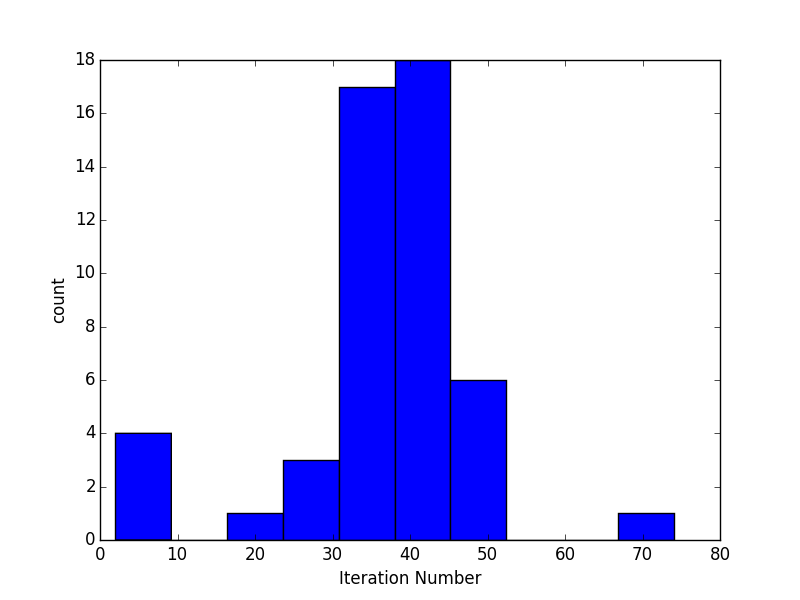
\includegraphics[scale = 0.6]{Iter_Histogram_random}
\end{center}
\subsection*{KMeans Initial Guess}
\begin{lstlisting}
def kmeans_estimate(x):
    labels = k_means(x,2)[1]
    # print labels
    cluster = [[],[]]
    for i in xrange(len(labels)):
        cluster[labels[i]].append(x[i])
    cluster[0] = np.array(cluster[0])
    cluster[1] = np.array(cluster[1])
    pi = len(cluster[0])*1.0/len(labels)
    pis = [pi,1-pi]
    means = []
    sigmas = []
    for i in xrange(2):
        curr = cluster[i]
        mean = np.average(curr,axis=0)
        means.append(mean)

        sigma = np.zeros((2,2))
        for i in xrange(len(curr)):
            y = np.reshape(curr[i]-mean, (2,1))
            sigma += np.dot(y, y.T)
        sigma /= len(curr)
        sigmas.append(sigma)

    pis = np.array(pis)
    means = np.array(means)
    sigmas = np.array(sigmas)
    print means
    return pis,means,sigmas
\end{lstlisting}
\begin{center}
	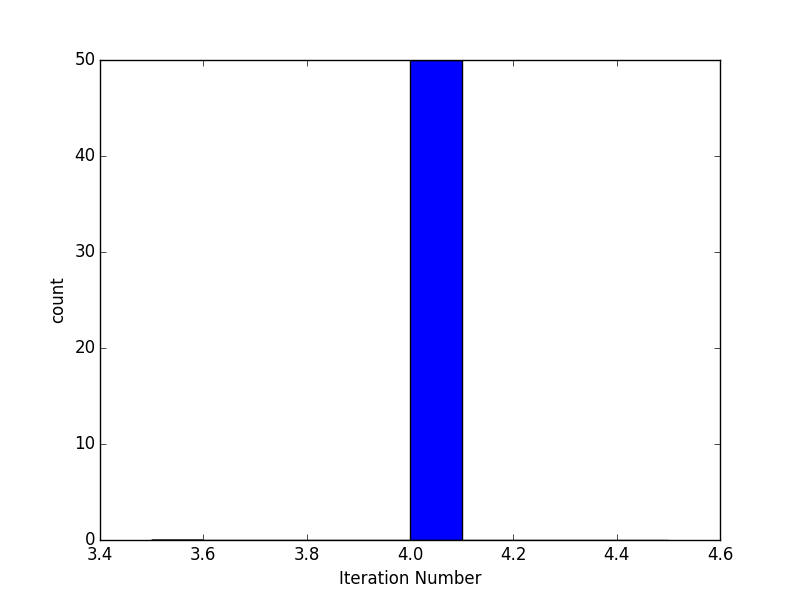
\includegraphics[scale=0.6]{Iter_Histogram_kmeans}
\end{center}
Compare with the random initialized guess, using KMeans can take very few steps for EM algorithm to converge. From the 2 histograms, random guess sometimes take 50 more iterations to converge but KMeans guess only take 4 iterations to converge. 
\end{document}